\setlength{\abovedisplayskip}{-25pt}
\setlength{\belowdisplayskip}{-25pt}

\section{Análise Teórica}

Antes de analisar cada um dos comparadores, vale destacar que o valor de saturação para ambos será igual, devido ao fato de que os AMPOPS estão sendo alimentados pelos mesmos níveis de tensão (+10V e -10V), assim os valores de saturação podem ser definidos como:

\begin{center}
\begin{equation} \label{vsat+}
       V_{sat}^{+} = + 10 V
\end{equation}
\end{center}

\begin{center}
\begin{equation} \label{vsat-}
       V_{sat}^{-} = - 10 V
\end{equation}
\end{center}

Já a entrada $V_{in}$ é controlada por um divisor de tensão em ambos os circuitos, sendo este composto por dois resistores de $10k\ohm$ e um potenciômetro de $15k\ohm$, de forma que a parcela do circuito pode ser redisposto como na figura \ref{div}. 

\begin{figure}[H]
\begin{center}
\begin{tikzpicture} [ american, ]
    %shorts
    \draw (0,0) node[left]{$+10V$} to[R, l=$10k \ohm$, o-] (2,0)
    (2,0) to[R, l=$15k \ohm - R_p$] (4,0)
    (4,0) to[R, l=$R_p$] (6,0)
    (6,0) to[R, l=$10k \ohm$, -o] (8,0) node[right]{$-10V$}
    (4,0) to[short, *-] (4,-1) node[left]{$V_{in}$}
    ;
    
\end{tikzpicture}
\end{center}
\caption{Divisor de tensão da entrada.}
\label{div} 
\end{figure}

Considerando que a resistência do resistor $R_p$ varia entre $0 \ohm$ e $15k \ohm$, tem-se que a tensão $V_{in}$ pode ser encontrada como:

\begin{center}
\begin{equation} \label{vin}
       V_{in} = -10 + 20 \times \frac{10^4 + R_p}{(10^4 + R_p) + (10^4 + 1.5 \times 10^4 - R_p)} = -10 + 20 \times \frac{10^4 + R_p}{3.5 \times 10^4} 
\end{equation}
\end{center}

Assim,  $V_{in} \in [-4.28,4.28]V$.

\subsection{Comparador não inversor simples}

Reconhece-se o circuito da figura \ref{ckt:1} como um comparador simples e não inversor. Isso pelo fato de possuir um valor de referência fixo ($V_{REF}=0V$) e que a tensão a ser comparada é inserida na entrada não inversora do AMPOP.

Assim, para que a saída $V_o$ esteja no nível positivo (+10V), basta que a tensão de entrada seja: $V_{in}>0V$. Para que a saída assuma o nível negativo (-10V), basta que a tensão de entrada seja: $V_{in}<0V$.

Dessa forma a característica de transferência do comparador pode ser considerada como a da figura \ref{graph:1}.


\begin{figure}[H]
\begin{center}
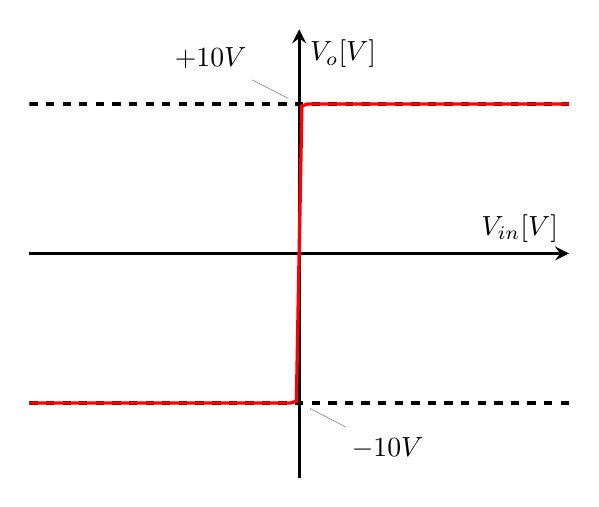
\begin{tikzpicture} 
\begin{axis}[very thick,
                     samples = 100,
                     ytick={-10,10},
                     xlabel = {$V_{in}[V]$},
                     ylabel = {$V_{o}[V]$},
                     xmin = -5,
                     xmax = 5,
                     ymin = -15,
                     ymax = 15,
                     axis x line = middle,
                     axis y line = middle,
                     ticks = none]
            \addplot[dashed] plot (\x, 10);
            \addplot[dashed] plot (\x,-10);
            \addplot[red] plot (\x, {-10+20/(1 + exp(-\x*100))});
            \addplot[mark=none] coordinates {(0,10)} node[pin=150:{$+10V$}]{};
            \addplot[mark=none] coordinates {(0,-10)} node[pin=-30:{$-10V$}]{};
        \end{axis}
\end{tikzpicture}
\end{center}
\caption{Característica de transferência para o comparador não inversor simples.}
\label{graph:1} 
\end{figure}

Finalmente, em relação aos LEDs, quando a saída assumir nível alto, o LED com catodo aterrado será ligado e o outro permanecerá apagado. Quando a saída assumir o nível baixo, o LED com catodo aterrado apagará e o outro acenderá.

\subsection{Comparador inversor com histerese}

Reconhece-se o circuito da figura \ref{ckt:2} como um comparador inversor com histerese. Isso é confirmado, pois o valor de referência é criado a partir de um divisor de tensão da tensão de saída por meio de uma malha de realimentação positiva e a tensão ser comparada é inserida na entrada inversora do AMPOP. Assim, as entradas do amplificador operacional em função da tensão de entrada e saída do do circuito comparador podem ser obtidas por meio das relações \ref{v+} e \ref{v-}

\begin{center}
\begin{equation} \label{v+}
       V^+ = V_{in}
\end{equation}
\end{center}

\begin{center}
\begin{equation} \label{v-}
       V^- = \frac{1.2 \times 10^3}{1.2 \times 10^3 + 12 \times 10^3} \times V_o = 0.0909 \times V_o
\end{equation}
\end{center}

Como é um comparador por histerese, deve-se encontrar os dois valores de transição. Dessa forma, considera-se inicialmente que para que a saída seja $V_o=+10V$, as entradas do AMPOP devem obedecer a seguinte relação: $V^+>V^-$. Desenvolvendo essa relação com base em \ref{v+} e \ref{v-}, tem-se a equação \ref{trans:1} que indica o primeiro valor de transição.

\begin{center}
\begin{equation} \label{trans:1}
       V_{in}<0.909 V
\end{equation}
\end{center}

Já o outro nível de transição pode ser obtido fazendo $V_o=-10V$, as entradas do AMPOP devem obedecer a seguinte relação: $V^+<V^-$. Desenvolvendo essa relação com base em \ref{v+} e \ref{v-}, tem-se a equação \ref{trans:2} que indica o segundo valor de transição.

\begin{center}
\begin{equation} \label{trans:1}
       V_{in}>-0.909 V
\end{equation}
\end{center}

Por fim, a característica de transferência do comparador inversor com histerese pode ser observado na figura \ref{graph:2}. 


\begin{figure}[H]
\begin{center}
\begin{tikzpicture} 
\begin{axis}[very thick,
                     samples = 100,
                     ytick={-10,10},
                     xlabel = {$V_{in}[V]$},
                     ylabel = {$V_{o}[V]$},
                     xmin = -5,
                     xmax = 5,
                     ymin = -15,
                     ymax = 15,
                     axis x line = middle,
                     axis y line = middle,
                     ticks = none]
            \addplot[dashed] plot (\x, 10);
            \addplot[dashed] plot (\x,-10);
            \addplot[red, name path=A] plot (\x, {-10+20/(1 + exp(-(-\x-0.909)*100))});
            \addplot[red, name path=B] plot (\x, {-10+20/(1 + exp(-(-\x+0.909)*100))});
            \addplot[mark=none] coordinates {(0,10)} node[pin=150:{$+10V$}]{};
            \addplot[mark=none] coordinates {(0,-10)} node[pin=-30:{$-10V$}]{};
            \addplot[->] coordinates {(0.909,0) (0.909,-0.0001)};
            \addplot[->] coordinates {(-0.909,-0.0001) (-0.909,0)};
            \addplot[mark=none] coordinates {(-0.909,0)} node[pin=150:{$-0.9V$}]{};
            \addplot[mark=none] coordinates {(0.909,0)} node[pin=-30:{$+0.9V$}]{};
        \end{axis}
        
\end{tikzpicture}
\end{center}
\caption{Característica de transferência para o comparador inversor com histerese.}
\label{graph:2} 
\end{figure}


Em relação aos LEDs, aquele que possui catodo aterrado só acenderá quando $V_{in}<-0.909V$, considerando que antes esteja apagado. Já o outro LED estará ligado e será apagado. Porém uma vez ligado, o LED de catodo aterrado só será apagado quando $V_{in}>0.909V$, assim, ligando o outro LED. Dessa forma, obedecendo o ciclo de histerese da característica de transferência.

